%\section{Anforderungen}

%Das zu entwickelnde Programm wird online per Java Servlets zur Verfügung gestellt. Als Webserver wird der %Tomcat eingesetzt. Folgende Funktionalitäten sollen umgesetzt weden:

%\begin{itemize}
%\item Loginsystem für Lernenden und Betreuer
%\item Grafische Oberfläche
%\item Eintragen von neuen Übungsaufgaben bestehend aus:
%	\begin{itemize}
%	\item Sachtext /Aufgabenstellung
%	\item Musterlösung(en)
%	\item Angabe von realen Datenbanken mit Testdaten
%	\item Einteilung in Kategorie
%	\end{itemize}
%\item Löschen und Bearbeiten von Übungsaufgaben
%\item Erstellen, Bearbeiten und Löschen von Kategorien
%\item Lösen von Übungsaufgaben durch Angabe einer SQL-Anfrage
%\item Tracking von Lösungsversuchen (Versuch, AufgabenID, Timestamp, UserID)
%\item Tracking von Usern und letzten Aktivitäten
%\item Tracking von Fehlern/ Fehlversuchen pro Aufgabe/User
%\end{itemize}

\section{Dokumentation}

Im folgendem Abschnitt beschreiben wir die Struktur des Programms und gehen, in übersichtlicher Form, auf die einzelnen Klassen und Funktionen des Programms ein. Eine noch detaillierte Fassung der Dokumentation findet sich im Quelltext als Javadocs-Kommentare.

\subsection{Datenbankstruktur}

Wir benutzen eine Datenbank um Aufgabenstellungen, Nutzer, Lösungsversuche und vieles mehr abzuspeichern. Im folgenden werden die einzelnen Tabellen erläutert. Wir verwenden dazu bewusst eine abstraktere Form der Beschreibung. Begründet ist dies, durch die Vielfalt der verschiedenen DBMS und ihrer verschiedenen Auslegung der Data Defintion Language. Im Prototypen verwenden wir das DBMS MySQL, man könnte aber alle DBMS verwenden, die einen JDBC Connector haben.

\textbf{attempts} (\underline{id}, userid $\to$ user(id), taskid $\to$ tasks(id), timeat ,sqlstatement ,correct)

Die Tabelle \verb|attempts| speichert je einen Lösungsversuch eines Benutzers. Dabei wird die SQL-Anfrage (\verb|sqlstatement|) eines Benutzers (mit der ID \verb|userid|) mit der Uhrzeit (\verb|timeat|) abgespeichert. Weiterhin wird vermerkt, welche Aufgabe (\verb|taskid|) der Student lösen wollte und, ob dieser Korrekt war.

\textbf{dbschema} (taskid $\to$ tasks(id), name, schema)

In der Tabelle \verb|dbschema| speichern wir zu jeder Aufgabe \verb|taskid|, wie die Struktur der Tabelle dafür aussieht. Wir speichern dazu, möglichst SQL-92 konforme, \verb|CREATE TABLE|-Anweisungen im Attribut \verb|schema|. Wir ordnen dem Schema außerdem einen Namen zu, damit es später einfach wiederzufinden ist.

\textbf{external\_database} (id, uri, dbname, username, password, typ)

Die Tabelle \verb|external_database| speichert die Zugriffsdaten (\verb|username,password|) einer externen Datenbank, die verwendet wird, um die notwendigen Bedingung einer Äquivalenz zu prüfen. Weiterhin speichern wir den Zugriffspfad auf diese Datenbank (\verb|uri|) und den Datenbanknamen (\verb|dbname|). Schließlich speichern wir noch den Typ. Im Moment werden mysql, postgresql und oracle als Typ unterstützt. Wir gehen später darauf ein, wie wir die Funktionalität auf noch mehr Datenbanken ausweiten können.

\textbf{samplesolutions} (id, taskid, sqlstatement)

Die Musterlösung für eine Aufgabe, wird in der Tabelle \verb|samplesolutions| gespeichert. Wir erfassen dabei die Aufgabennummer (\verb|taskid|), sowie die Musterlösung als SQL-Anfrage (\verb|sqlstatement|). Wir verwenden einen künstlichen Schlüssel \verb|id|, da es unter Umständen mehrere Musterlösungen zu einer Aufgabe geben kann.

\textbf{tasks} (id, description, respectColumnOrder, schemaid, createdAt$^0$)

Die Aufgaben werden in der Tabelle \verb|tasks| gespeichert. Wir versehen jede Aufgabe mit einer \verb|id| und einer Beschreibung, in Form eines Sachtextes (\verb|description|). Wir speichern, ob die Reihenfolge der Spalten (im \verb|SELECT|-Teil) eingehalten werden muss und, erfassen außerdem, welches Datenbankschema zu dieser Aufgabe zugeordnet werden soll. Optional können wir noch vermerken, wann die Aufgabe eingetragen wurde.

\textbf{tasks\_db} (taskid $\to$ tasks(id), dbid $\to$ external\_database(id))

Es kann unter Umständen möglich sein, pro Aufgabe mehrere externe Datenbanken anzugeben. Daher speichern wir die Zuordnung einer Datenbank zu einer Aufgabe in der Tabelle \verb|tasks_db|. Hierzu verwenden wir den Fremdschlüssel zur Aufgabentabelle (\verb|taskid|) und den zur externen Datenbank (\verb|dbid|).

\textbf{users} (id, name, password, isDozent)

Einzelne Benutzer werden in der Tabelle \verb|users| erfasst. Neben den üblichen Kontoinformationen, wie \verb|name, password| speichern wir auch, ob der Nutzer ein Dozent ist. Diese Information ist wichtig, um zu entscheiden, ob ein Nutzer auch Aufgaben einpflegen darf.

\subsection{Programmstruktur}

In diesem Abschnitt werden wir die wichtigsten Klassen und Funktionen auflisten und erläutern. Eine vollständige Dokumentation aller Klassen, ist im Quellcode als Javadocs-Kommentare vorhanden. (TODO: evt Anhang).

Das Programm beinhaltet mehrere Prozesse, die sich aus der Abfolge mehrere Funktionen zusammensetzen. Im Folgenden werden alle wesentlichen Prozesse und deren Zusammensetzung erläutert. Wir gehen dabei auch auf Möglichkeiten zur Anpassung des Programms ein.

\subsubsection{Prozess: Standardisieren einer SQL-Anfrage} 

Wir beschäftigen uns zu erst mit einer der Hauptfunktionen: das Standardisieren einer SQL-Anfrage. Die Klasse \verb|QueryHandler| kümmert sich um das Standardisieren einer SQL-Anfrage. Für jede SQL-Anfrage wird ein separates Objekt dieser Klasse erzeugt. Anschließend importieren wir das, zu Grunde liegende, Datenbankschema in das Objekt. Dies geschieht mit der Methode: \\\verb|boolean createTable(String createTableStatement)|\\
Die Methode erwartet pro Aufruf ein, wenn möglich SQL-92 konformes, \verb|CREATE TABLE|-Statement. Nachdem wir das Datenbankschema eingelesen haben, importieren wir noch die zu standardisierende Anfrage. Dies geschieht mit der Methode:\\\verb|setOriginalStatement(String s)|\\ Das eingegebene Statement wird dann mit Hilfe des ZQL-Parsers eingelesen. Etwaige Fehler beim Parsen werden per Exception an den Nutzer weitergereicht. Mehr dazu im Abschnitt >>Webinterface<<. Wir kopieren das Statement außerdem, so dass wir intern zwei ZQuery-Objekte speichern, zum einen die Originalanfrage im Objekt \textbf{original}, die niemals verändert wird, zum Anderen eine Arbeitskopie im Objekt \textbf{workingCopy}, welche wir dann standardisieren. Nun ist das Datenbankschema eingelesen und die, zu verarbeitende, Anfrage liegt vor. Wir können den Standardisierungsprozess nun starten, mit der Methode: \\\verb|ZQuery[] equalize(boolean respect)|\\ 
Als Eingabeparameter erhält sie die Information, ob die Reihenfolge im \verb|SELECT| respektiert werden soll, oder nicht. Im Abschnitt >>externe Datenbanken<< haben wir bereits darüber diskutiert, dass diese Funktion durchaus interessant sein kann. Weiterhin beobachten wir, dass die Methode nicht eine Anfrage, sondern ein Array von Anfragen zurückliefert. Wir erinnern uns an die Problematik der Selbstverbunde. Dort werden mehrere Permutationen der Tabellen unter \verb|FROM| auf die Anfrage angewandt. Es entstehen dann mehrere Anfragen, die alle semantisch äquivalent sind, aber Aufgrund ihrer unterschiedlichen Struktur alle, mit der Lösung des Lernenden abgeglichen werden müssen.

Die Funktion \verb|equalize| startet die Funktion:\\
\verb|handleQUERY(ZQuery q)|\\Zu beachten ist der Parameter. Da die Abfrage während des Standardisierens verändert wird, ist die ursprüngliche Anfrage des Studenten, unwiederbringlich, verändert. Damit dies nicht geschieht, entscheiden wir nun welche Anfrage zum Standardisieren übergeben wird. Wir übergeben hier das Objekt \textit{workingCopy}.

\verb|handleQUERY| speichert zunächst alle Metainformationen der Anfrage in einem Objekt der Klasse \verb|MetaQueryInfo|. Wie dies genau geschieht behandeln wir später, in diesem Kapitel. Anschließend verarbeitet \verb|handleQUERY| mit Hilfe der Methode:\\
\verb|handleFROM|\\
den \verb|FROM|-Teil unserer Anfrage. Die Verarbeitung hängt vom \verb|SELECT|-Teil ab. Wie bereits in Kapitel \ref{chap:theorie} besprochen, werden, abhängig vom \verb|SELECT|-Teil, die Tabellen zunächst sortiert. Anschließend erhalten alle Tabellen einen künstlichen Alias, der fortlaufend ist. In der Standardeinstellung des Programmes ist dies \verb|a1, a2, a3, ...| Die verwendeten Aliase werden nun in einer \textit{HashMap} als Attribut \textbf{Zuordnung} in der Klasse QueryHandler gespeichert. 

Anschließend bearbeiten wir den \verb|SELECT|-Teil unserer Anfrage mit der Funktion:\\
\verb|Vector<ZSelectItem> handleSELECTClause(Vector<ZSelectItem> sel)|\\
Im wesentlichen ändern wir hier vorhandene Aliase in unsere automatisch erzeugten. Finden wir dabei Attribute, die keine Aliase besitzen und es mehrere Tabellen unter \verb|FROM| gibt, die dieses konkrete Attribut beinhalten, lösen wir eine Fehlermeldung aus, wegen Uneindeutigkeit.

Jetzt erstellen wir Permutationen der Tabellen in der \verb|FROM|-Liste. Wir gehen dabei vor, wie im Kapitel \ref{chap:theorie} beschrieben. Sind in unter \verb|FROM| keine zwei gleichen Tabelle, dann enthält die Menge der Permutationen nur die ursprüngliche Anordnung. Die nun folgenden Schritte werden für jede permutierte \verb|FROM|-Liste durchgeführt.

\verb|equalize| fährt fort mit der Methode: \verb|ZExp handleWHERE(ZExp exp)|.\\
Innerhalb dieser Methode erledigen wir alle Arbeiten, die im Abschnitt >>WHERE-Teil<< in Kapitel \ref{chap:theorie} erläutert wurden. Zunächst führen wir die künstlichen Aliase ein mit der Funktion \verb|makeAlias|. Dies geschieht in ähnlicher Weise, wie im \verb|SELECT|-Teil. \verb|makeAlias| sucht auch nach Unterabfragen. Findet es solche, werden diese ersetzt durch ihre standardisierte Form, indem der Standardisierungsprozess für diese rekursiv aufgerufen wird. Danach transformieren wir, mit der Funktion \verb|transformToKNF|, die aktuelle Form des \verb|WHERE|-Ausdrucks in eine konjunktive Normalform. Dabei bedient sich \verb|transformToKNF| der Funktionen:\\
\verb|operatorCompression, pushDownNegate| und \verb|distribute|. Die Vorgehensweise entspricht der besprochenen im theoretischen Bereich dieser Arbeit. Wir ersetzen danach Unterabfragen durch \verb|EXISTS|-Unterabfragen, wenn möglich. Anschließend werden implizite Formeln hinzugefügt sowie arithmetische und logische Ausdrücke ausgewertet, soweit dies möglich ist. Gerade durch die letzten, beiden Teilschritte, kann es passieren, dass die konjunktive Normalform wieder zerstört worden ist. Daher wenden wir an dieser Stelle erneut \verb|transformToKNF| an. Als letzten Schritt sortieren wir den Ausdruck so, wie ausführlich im Bereich \ref{subsec:sort} beschrieben. Die Sortierung beinhaltet auch die Duplikateliminierung bei doppelten \verb|AND|- oder \verb|OR|-Operanden.

\verb|handleQUERY| wendet sich jetzt dem \verb|GROUP BY|-Teil zu. Dieser wird in zwei Teilen abgearbeitet. ZQL trennt \verb|GROUP BY|- vom \verb|HAVING|-Teil. Im \verb|GROUP BY|-Teil sortieren wir lediglich lexikographisch, wie schon im \verb|SELECT|-Teil. Der \verb|HAVING|-Teil wird mit der Funktion \verb|handleWHERE| behandelt, da sich beide Ausdrücke strukturell gleichen.

Der entstandene SQL-Ausdruck, in Form eines \verb|ZQuery|-Objektes, wird von \verb|handleQUERY| direkt zu \verb|equalize| zurückgeliefert. Der Standardisierungsprozess ist damit beendet. Abbildung \ref{fig:execPlan} soll die Reihenfolge der abgearbeiteten Funktionen noch einmal verdeutlichen. Schwarze Pfeile bedeuten eine iterative Abarbeitung und blaue Pfeile bedeuten Unterprogrammabrufe innerhalb einer Methode.

\begin{figure}[h]
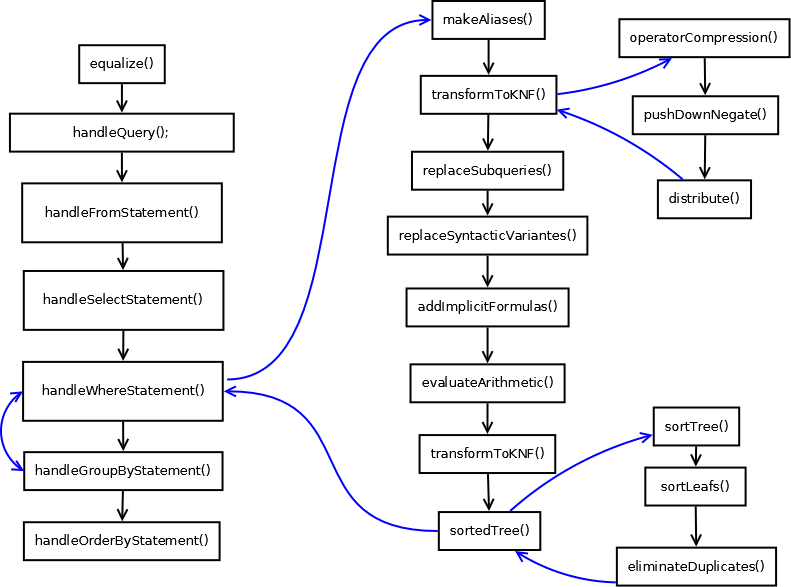
\includegraphics[scale=0.39]{Bilder/execPlan.png}
\caption{Einfacher Programmablaufplan}
\label{fig:execPlan}
\end{figure}

\subsubsection{Prozess: Verwenden von externen Datenbanken} 


\subsection{Webinterface}

Das Programm soll, mit Hilfe der Java Server Pages (JSP), als Webseite darstellbar sein. 

\subsection{Externe Datenbanken}


\subsection{Technische Details}

Die Umsetzung einiger, in Kapitel \ref{chap:theorie}, Sachverhalte ist in der Praxis etwas komplexer, als theoretisch erdacht. Im Folgenden Abschnitt gehen wir daher auf Implementierungsdetails einiger Funktionen ein, die sich etwas komplexer gestalten. Es soll damit ein Eindruck vermittelt werden, wie die theoretischen Sachverhalte in ein konkretes Programm übertragbar sind.

